\documentclass[12pt]{article}
\usepackage[english]{babel}
\usepackage{natbib}
\usepackage{url}
\usepackage[utf8x]{inputenc}
\usepackage{amsmath}
\usepackage{graphicx}
\graphicspath{{images/}}
\usepackage{parskip}
\usepackage{fancyhdr}
\usepackage{vmargin}
\setmarginsrb{3 cm}{2.5 cm}{3 cm}{2.5 cm}{1 cm}{1.5 cm}{1 cm}{1.5 cm}

% Template started from: https://www.overleaf.com/latex/templates/uct-report-template/grctkzjtrqrm

\title{Course Project}										% Title
\author{Grant Atkins\\David Haslam}							%Authors
\date{\today}											% Date

\makeatletter
\let\thetitle\@title
\let\theauthor\@author
\let\thedate\@date
\makeatother

%\pagestyle{fancy}
%\fancyhf{}
%\rhead{\theauthor}
%\lhead{\thetitle}
%\cfoot{\thepage}

\begin{document}

%%%%%%%%%%%%%%%%%%%%%%%%%%%%%%%%%%%%%%%%%%%%%%%%%%%%%%%%%%%%%%%%%%%%%%%%%%%%%%%%%%%%%%%%%

\begin{titlepage}
	\centering
    \vspace*{0.5 cm}
    
\includegraphics[scale = 1.8]{ODU.png}\\[1.0 cm]	% University Logo
    \textsc{\LARGE Old Dominion University}\\[2.0 cm]	% University Name
	\textsc{\Large CS 773}\\[0.5 cm]				% Course Code
	\textsc{\large Data Mining and Security}\\[0.5 cm]				% Course Name
	\rule{\linewidth}{0.2 mm} \\[0.4 cm]
	{ \huge \bfseries \thetitle}\\
	\rule{\linewidth}{0.2 mm} \\[1.5 cm]
	
	\begin{minipage}{0.4\textwidth}
		\begin{flushleft} \large
			\emph{Authors:}\\
			\theauthor
			\end{flushleft}
			\end{minipage}~
			\begin{minipage}{0.4\textwidth}
			\begin{flushright} \large
%			\emph{Student Number:} \\
%			XXXXXX000									% Your Student Number
		\end{flushright}
	\end{minipage}\\[2 cm]
	
	{\large \thedate}\\[2 cm]
 
	\vfill
	
\end{titlepage}

%%%%%%%%%%%%%%%%%%%%%%%%%%%%%%%%%%%%%%%%%%%%%%%%%%%%%%%%%%%%%%%%%%%%%%%%%%%%%%%%%%%%%%%%%

\tableofcontents
\pagebreak

%%%%%%%%%%%%%%%%%%%%%%%%%%%%%%%%%%%%%%%%%%%%%%%%%%%%%%%%%%%%%%%%%%%%%%%%%%%%%%%%%%%%%%%%%

\section{Executive Summary}

The goal of this course project, originally stemmed from Open University Learning Analytics data set, is to identify ``at-risk'' students 
provided \cite{oulad}.

More needs to be done in this section...

%This is a simple report template with the UCT logo. Feel free to use/modify it to suit your needs. Variables that need to be altered have been commented to make modifications easier. For example if you need to change the university logo, look for the comment \texttt{\% University Logo} in this file and then make appropriate modifications in that line.
%
%A Table of Contents and a bibliography have also been implemented. To add entries to your bibliography, simply edit \texttt{biblist.bib} in the root folder and then use the \texttt{\textbackslash cite\{\ldots\}} command in \texttt{main.tex} \cite{bibtex}. The Table of Contents will be updated automatically.
%
%I hope that you find this template both visually appealing and useful. \\

\section{Introduction}

With analytics becoming an integral part of Learning Management Systems (LMS), Universities can analyze their data to intervene and aid ``at-risk'' 
students. This can be done by detecting failing or struggling students earlier on in their courses. These detections can later be used to predict ``at-risk''
students for future intervention. Analysis of demographic information for students may also prove useful to detect environments or character
attributes that identify a struggling group.

The Open University (OU) in the United Kingdom, offered distance learning courses with its virtual learning environment (VLE) from 2013 to 2014. Students interacted with 
the VLE and OU then collects information such as: page names, clicks, and times connected to the website. Students are also required to register for these 
courses earlier on, which provides: registration date, unregistration date, class types and semester. Many students may end up failing or withdrawing from the VLE 
courses. The data sets that OU provided can be used to provide insight on 2013 to 2014 semester students. 

\section{Problem Statement}

When analyzing students to observe for ``at-risk'' students it may seem easily done by looking at simply grade scores, however, there could be factors
present in a student's personal history or personal accomplishments that correlate with course problems causing a student to be ``at-risk.'' The goal of this paper is discuss and find data mining techniques that aid in the detection and prediction of ``at-risk'' students.

\section{Solution Methodology}

Finding a solution for this project was based on the data being observed. We first attempted to look at each data set, each csv provided, individually and then find attributes that would be the best indicators to determine the ``final\_result'' of students. The tools used for this project included weka and R. Later we would merge the data sets together and then perform the following steps depending on the data set:

\begin{enumerate}
  \item Find the best attributes for the data provided, often through information gain for feature selection or PCA for clustering
  \item Test machine learning techniques such as:
  \begin{enumerate}
     \item Decision trees
     \item Naive bayes
     \item Bagging
     \item K-means
  \end{enumerate}
  \item Cross validation for measuring effectiveness
\end{enumerate}

This paper first experiments upon the individual data sets and then the results of the merged data sets as explained in the next section.

\section{Experimental setup and data used}

There are many different ways to experiment on the OU learning analytics data set. There are many interactions between the different sets of data, such as demographic
information can be linked to course assessments for each student as shown in Figure \ref{fig:db_model}. The attribute ``final\_result'' was the main attribute that was used in each data set because it determines whether students passed, failed, withdrawn or gained distinction. We found these attributes to be along the same lines, so we eventually paired them to Pass or Fail, where withdrawn became Fail and distinction became Pass.

 \begin{figure}[h]
 \centering
 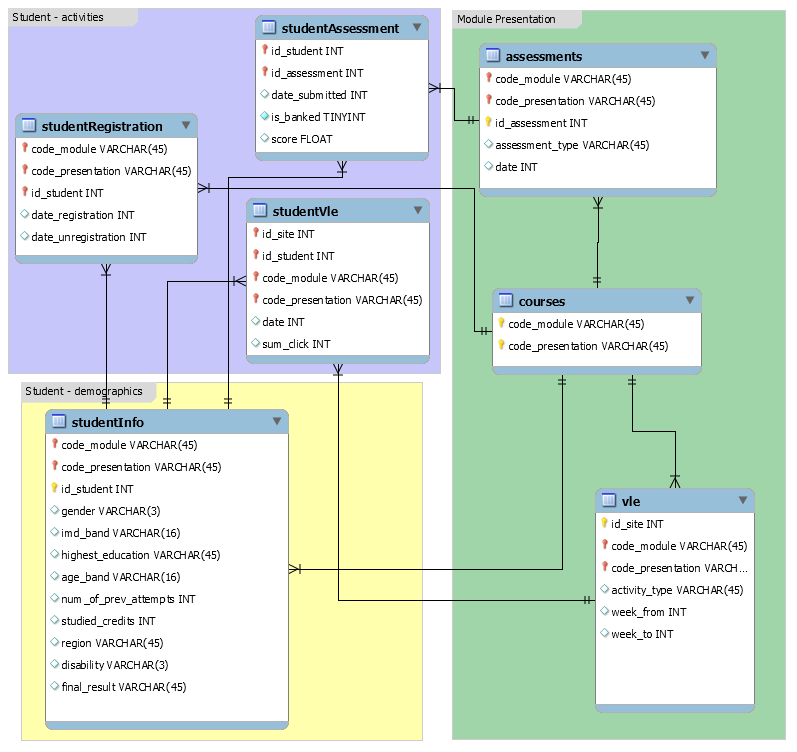
\includegraphics[scale=0.5]{db_model.png}
 \caption{OU learning analytics data set relations \cite{oulad}}
 \label{fig:db_model}
 \end{figure}
 
 \newpage
 While each file may contain valuable information about a student, many times important details can be lost among large amounts of useless data. In our attempt to isolate the most important attributes, we ran the files that were correlated with a student passing or failing to find information gain. These four files, "studentAssessment", "studentInfo", "studentRegistration", and "studentVle" provided the most useful attributes to determine if a student passed or failed. The information gain for each of these files is displayed below in Figure xx. We found that the files "course" and "Vle" were almost completely useless. 

 When later testing this data, non-important attributes were purged. For example, student\_id was removed because there is nothing to gain from specific individual students compared to other attributes such as score or code\_module where there can be correlations.

 After purging useless material from the input, we used various data mining techniques on each file separately to see if we could accurately predict whether a student would pass or fail. While certain files such as "studentVle" and "studentAssessment" did produce good results, it was not until we combined several of these files that we observed the best outcome.  
 
 In order to simplify the data, we only predict for two outcomes; pass and fail. The project states that we need to identify when a student needs counseling and are in danger of failing. Predicting for distinction would be useless because this is equivalent to passing. In addition, the main reasons for withdrawing is due to poor grades and lack of knowledge of the information. If a student was withdrawing, counseling would still be important and could possibly reverse the students decision.

\begin{figure}[h]
 \centering
 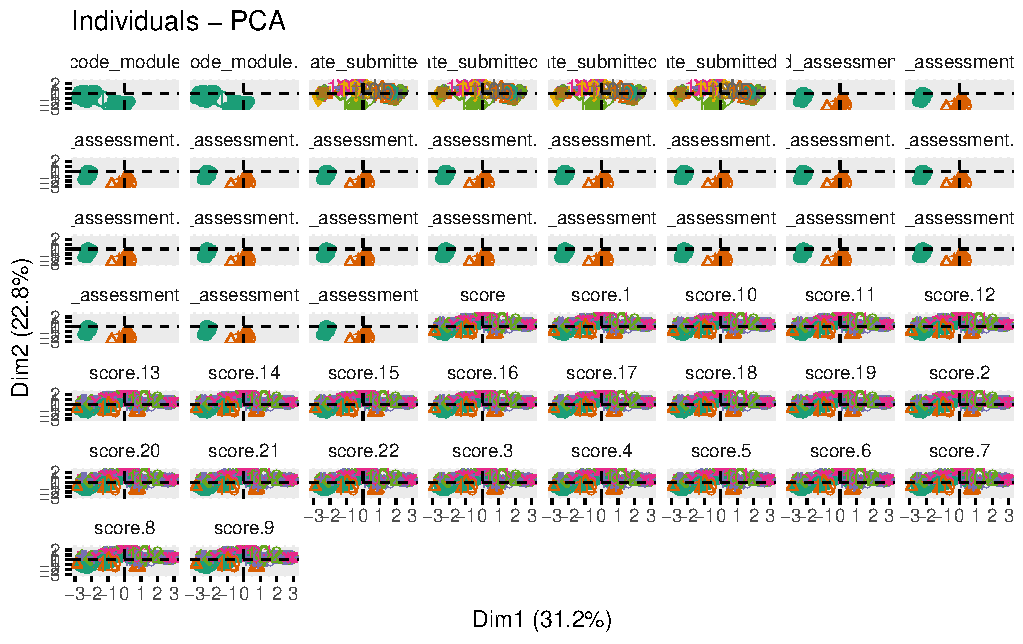
\includegraphics[scale=0.8]{PCA_Assessments_first50.pdf}
 \caption{PCA of student assessment attributes}
 \label{fig:pca}
 \end{figure}
 
 When first reviewing the data presented to us individually, student demographics was the first to be reviewed as this is information that is often received before a course has started. Approaching this set of data we first decided to use information gain to discover the best attributes to build a decision tree. This lead to interesting results as all of the attributes never had above a 5\% information gain as shown in table \ref{table:dem_infogain}. This deterred us away from using attributes from demographic information aside from final\_result, which is the classifier for this data set.
 
 
 \begin{table}
\centering
\begin{tabular}{ | l | l | l | p{7.8cm} | }
\hline
\textbf{Attribute} & \textbf{Information Gain} \\
\hline
code\_module & 0.0333132948 \\
\hline
studied\_credits & 0.0291538626 \\
\hline
highest\_education & 0.0220755496 \\
\hline
imd\_band & 0.0190484622 \\
\hline
date\_registration & 0.0126263112 \\
\hline
num\_of\_prev\_attempts & 0.0112197577 \\
\hline
region & 0.0099021067 \\
\hline
code\_presentation & 0.0090550367 \\
\hline
age\_band & 0.0047750479 \\
\hline
disability & 0.0030386879 \\ 
\hline
gender & 0.0003658152 \\
\hline

\end{tabular}
\caption{Information gain of student info and registration data merged}
\label{table:dem_infogain}
\end{table}

\section{Results}

Performing simple k-means using Weka's ``densityBasedClusterer'', showed very clear cluster when observing a students' click counts vs students' assessment scores as shown below in Figure \ref{fig:click_vs_score}.
K-means chose number of clicks as the best attribute to perform clustering on.

\begin{figure}[h]
 \centering
 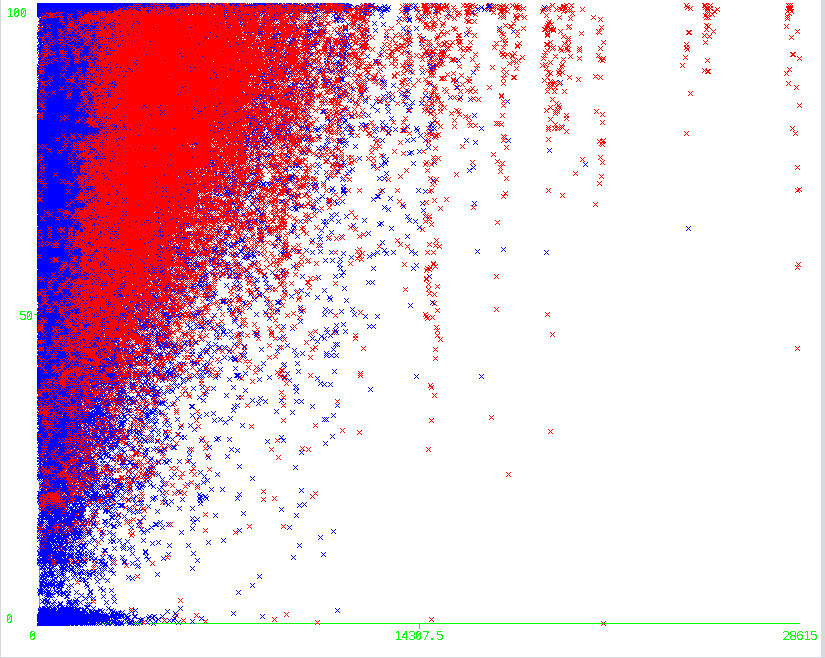
\includegraphics[scale=0.35]{click_count_vs_score_clusters.png}
 \caption{K-means clusters for click\_counts vs scores}
 \label{fig:click_vs_score}
 \end{figure}
 
 \begin{figure}[h]
 \centering
 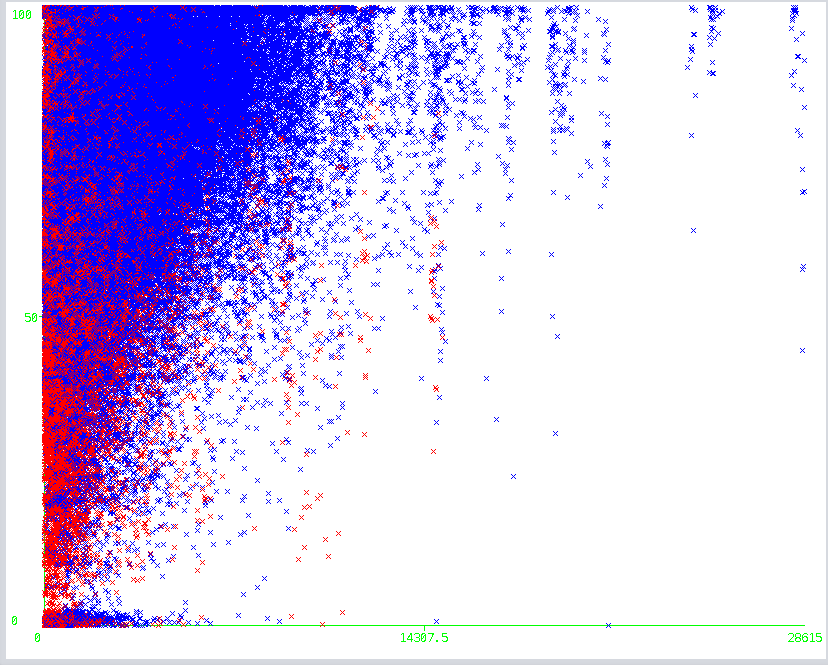
\includegraphics[scale=0.35]{click_count_vs_score_finalresults.png}
 \caption{K-means results for click\_counts vs scores with Blue being passing and red being failing}
 \label{fig:click_vs_score_f}
 \end{figure}

 
 If we view the clusters as final results, it becomes apparent that there is a correlation between click counts and scores for determining if a student passes or fails in the end. After approximately 14,500 clicks in the content, students generally all pass, even if a student receives a failing score after as shown in Figure \ref{fig:click_vs_score_f}.


\begin{figure}[h]
 \centering
 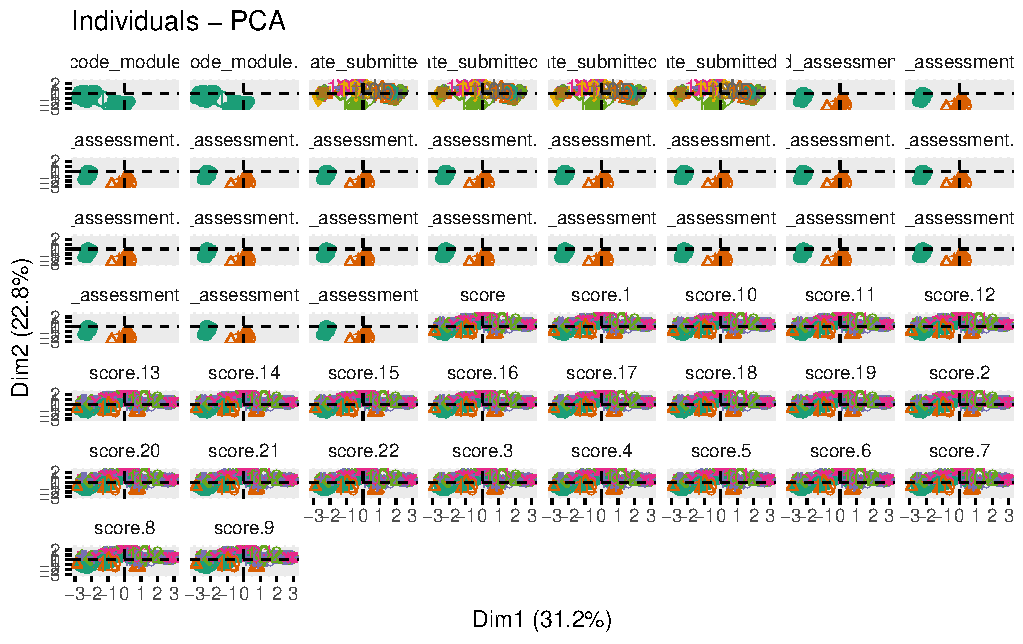
\includegraphics[scale=0.8]{PCA_Assessments_first50.pdf}
 \caption{PCA of student assessment attributes}
 \label{fig:pca}
 \end{figure}

Students who took the highest weighted assignment, where weight was 100, and scored below a 50 had a 87.88\% chance to fail. This is fairly critical making students

Students who logged in to the VLE before the course started had a 67\% chance to pass. 

\clearpage
\section{Conclusions}s.



%\hspace{1 cm}--- End

\clearpage
\bibliographystyle{plain}
\bibliography{biblist}

\end{document}